\documentclass[a4paper,12pt]{article}
\author{Geoffrey Gaillard et Thomas Jeantet}
\usepackage[french]{babel}
\usepackage{amsmath}
\usepackage{graphicx}
\usepackage{amsfonts}
\usepackage{pdflscape}
\usepackage[utf8]{inputenc}
\usepackage{float}



%Package
\usepackage[margin=1in]{geometry}
\usepackage{fancyhdr}
\usepackage{placeins}
\usepackage{listings}
\usepackage{color}
\usepackage[table,xcdraw]{xcolor}
\usepackage{ulem} %barrer du texte
\usepackage{cancel}% barrer dans une expression math (\cancel{})
\usepackage{pgf,tikz}
\usepackage{mathrsfs}
\usepackage{multirow}
%\usepackage{gensymb}
\usepackage{caption}
\usepackage{eurosym}% pour le symbole €



\usetikzlibrary{shapes.geometric, arrows}
\definecolor{qqqqff}{rgb}{0.,0.,1.}
%Configuration
\renewcommand*\contentsname{Sommaire}
\graphicspath{ {images/} }
%\renewcommand{\thesection}{\Roman{section}}
%\renewcommand{\thesubsection}{\Alph{subsection}}

\definecolor{codegreen}{rgb}{0,0.6,0}
\definecolor{codegray}{rgb}{0.5,0.5,0.5}
\definecolor{codepurple}{rgb}{0.58,0,0.82}
\definecolor{backcolour}{rgb}{0.95,0.95,0.92}
 
\lstdefinestyle{mystyle}{
    backgroundcolor=\color{backcolour},   
    commentstyle=\color{codegreen},
    keywordstyle=\color{magenta},
    numberstyle=\tiny\color{codegray},
    stringstyle=\color{codepurple},
    basicstyle=\footnotesize,
    breakatwhitespace=false,         
    breaklines=true,                 
    captionpos=b,                    
    keepspaces=true,                 
    numbers=left,                    
    numbersep=5pt,                  
    showspaces=false,                
    showstringspaces=false,
    showtabs=false,                  
    tabsize=2
}

\lstset{style=mystyle}
\renewcommand{\lstlistingname}{Script}

\date{15 Juin 2016}

\pagestyle{fancy}
\fancyhf{}
\rhead{Geoffrey Gaillard et Thomas Jeantet}
\lhead{IF23 - Système de géolocalisation embarqué}
%\rfoot{Page \thepag}










\title{Projet IF23\\Etude d'un système de géolocalisation}
\date{15 Juin 2016}
\graphicspath{{/home/apache/Documents/UTT/SRT2/IF23/IF23-Project/src/data/itinary_1/}{/home/apache/Documents/UTT/SRT2/IF23/IF23-Project/src/data/itinary_2/}{/home/apache/Documents/UTT/SRT2/IF23/IF23-Project/src/data/itinary_3/}{/home/apache/Documents/UTT/SRT2/IF23/IF23-Project/src/data/itinary_4/}}
\begin{document}
\maketitle
\newpage
\tableofcontents
\newpage


\section*{Avant-Propos}
Depuis la première mise en service à la fin des années 60, les systèmes de positionnement par satellites n'ont cessé d'être améliorés. Leur utilisation a grandement facilité la navigation, qu'elle soit terrestre, maritime, aérienne ou parfois même spatiale. Dans le cadre de ce projet, nous avons pu programmer un système GPS embarqué et étudier la précision de ce système de positionnement. Ce système GPS est constitué d'une Arduino Micro Pro, d'un recepteur GPS, d'un écran LCD, d'une carte mémoire micro SD et de 4 boutons. L'intégralité du code source est disponible à l'adresse suivante: https://github.com/Vanell/IF23-Project .
\section{Fonctionnalités du système GPS}
Notre programme permet au boitier, outre de récupérer les données GPS, d'afficher sur l'écran LCD les informations suivantes:
\begin{itemize}
\item Latitude
\item Longitude
\item Nombre de satellites visibles
\item HDOP
\item Altitude
\item Vitesse
\item Date
\item Heure GPS
\item Tension de la batterie
\item Autonomie en heures
\item Pourcentage de charge de la batterie

\end{itemize}

De plus, l'utilisateur peut accéder à un menu pour prendre un point ou lancer la prise d'itinétaire.
En parallèle de la programmation du système GPS, nous avons développé un programme en python qui permet de:
\begin{itemize}
\item Récupérer les données enregitrées sur la carte SD via le port série
\item Mettre les données en forme et leur appliquer une correction Lambert 93
\item Calculer les précisions relatives à une mesure
\item Gérer les fichiers présents sur la carte SD
\item Exporter les données en format .csv et en .gpx

\end{itemize}
\newpage
\section{Utilisation du système}
L'interface utilisateur se découpe en deux partie: l'affichage des données GPS en temps réel, et le menu de prise de points. Les deux boutons de gauche servent à naviguer dans les affichage, tandis que les deux boutons de droite servent à passer d'un type d'affichage à l'autre. L'utilisation des quatre boutons, de gauche à droite, est:\newline
Monter dans le menu, descendre dans le menu, affichage des information relatives à l'autonomie ou retour au données temps réel, ouverture du menu de prise de points ou validation. \\
Pour une vision plus claire de l'interface, voir le diagramme de cas d'utilisations en figure 1.

\begin{figure}[!ht]
	\begin{center}
		
		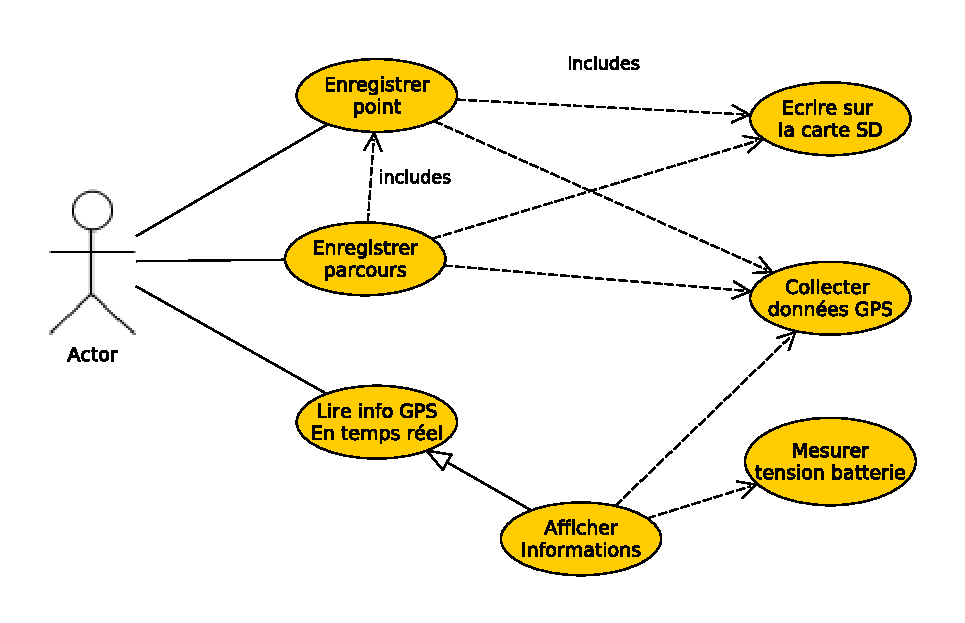
\includegraphics[scale = 0.9]{UseCase.eps}
		\caption{Diagramme de cas d'utilisation}
	\end{center}
\end{figure}
\FloatBarrier
\newpage
\section{Description fonctionnelle}
Pour nous faciliter le travail de développement, nous avons utilisé des bibliothèques de fonctions déjà existantes, dont voici la liste exhaustive:
\begin{itemize}
\item TinyGPS, bibliothèque de traitement de données brutes GPS
\item SoftwareSerial, pour effectuer la liaison serial avec le recepteur GPS
\item avr/pgmspace, permettant de stocker des variables dans la mémoire flash de l'arduino
\item Bounce2, pour éviter de capter les rebonds des boutons poussoir
\item LiquidCrystal, facilitant l'utilisation de l'écran LCD
\item SD, bibliothèque native d'Arduino permettant de créer des objets\\ ``File'' et de les enregistrer
\end{itemize}

Lors du dévelopement, nous avons décidé de découper notre programme en plusieurs ``bibliothèques'' de fonctions Arduino, chacune orientée sur un aspect du programme du système.
\subsection{Bibliothèque GPS}

Cette bibliothèque de fonctions nous permet de définir les variables globales liées au GPS (comme un booléen indiquant si les données GPS ont changé), ainsi que la fonction de mise à jour des coordonnées GPS. Cette dernière récupère toutes les données fournies par la bibliothèque TinyGPS, et les stocke dans un tableau.
\subsection{Bibliothèque d'affichage}

L'affichage sur l'écran LCD est géré par trois fonctions: la première permet de détecter l'appui sur un bouton, et détermine quel bouton a été pressé. La deuxième incrémente ou décrémente des valeurs dans un tableau pour savoir quelles données afficher. Enfin, la troisième fonction lit les valeurs dans ce tableau, et met les données de l'écran à jour. C'est également dans cette fonction que l'on pourra décider de prendre un point ou un itinéraire.
\subsection{Bibliothèque SD}

A partir de la bibliothèque native d'Arduino permettant d'écrire et lire sur une carte SD, nous avons codé des fonctions permettant d'écrire toutes les données GPS instantanées sur un fichier ou de lire un fichier et d'écrire son contenu sur le port série. Nous avions aussi prévu de lister les fichiers présent sur la carte SD, mais cette option n'a pas pu être implémentée faute de place sur l'Arduino.

\newline

En figure 2 se trouve l'algorithme de la fonction \textit{loop}. Les algorithmes des bibliothèques que nous avons développé ne sont pas détaillées ici, car il sont relativement simples et ne présentent pas grand intérêt.
\newpage
%\begin{landscape}
\begin{figure}[!ht]
	\begin{center}
		
		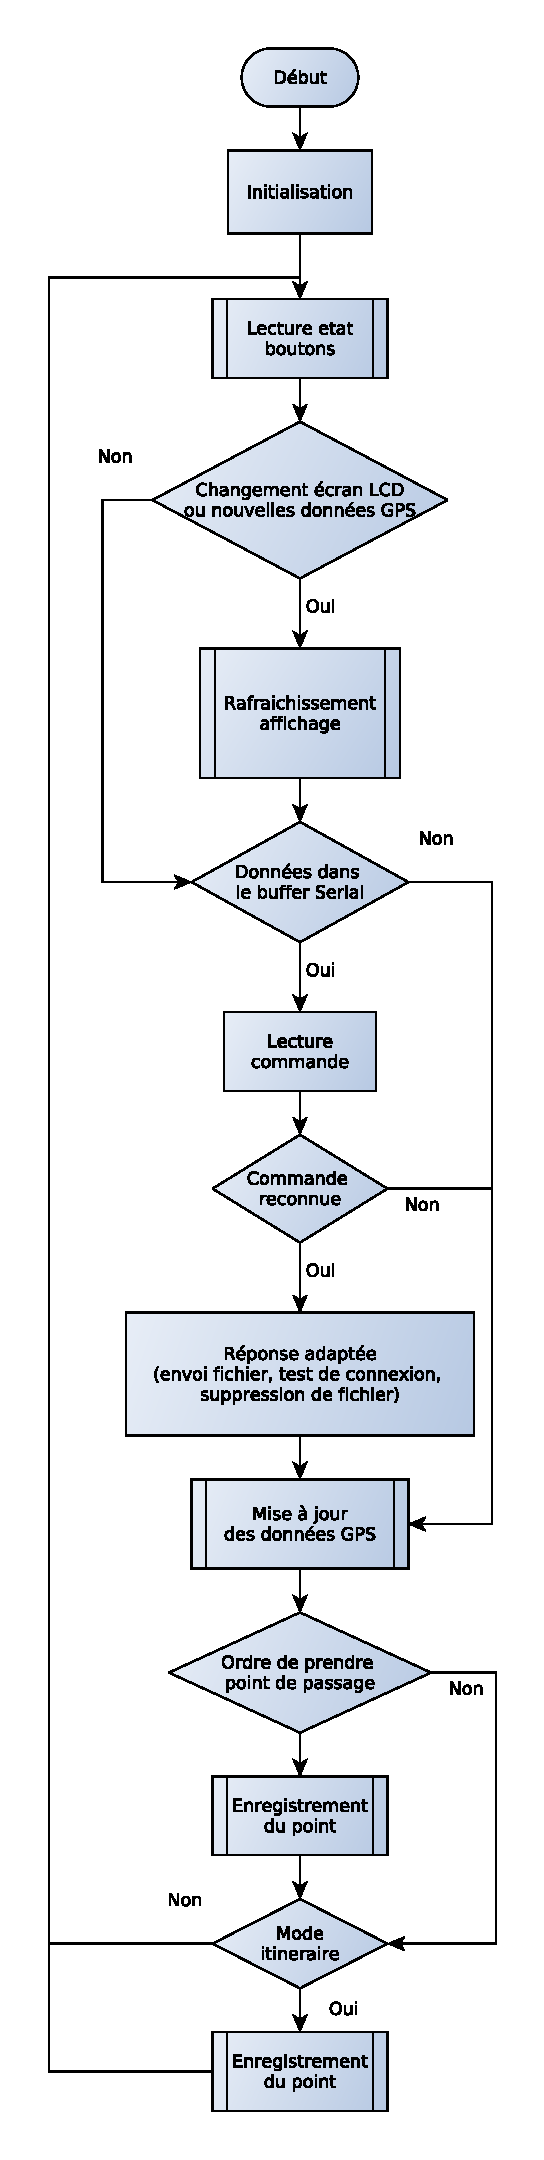
\includegraphics[scale = 0.5]{MainAlgoGraph.eps}
		\caption{Boucle principale}
	\end{center}
\end{figure}
\FloatBarrier

\newpage

\section{Traitement et interprétation des données}
Nous avons effectué 4 séries de mesures utilisables, chacune dans un lieu différent. Le choix de ces endroits nous a semblé crucial car les mesures prises nous permettront d'estimer les paramètres influençant la précision du GPS. Pour mieux comprendre l'interprétation des résultats, voici une brève description des lieux:
\begin{itemize}
\item Appartement au 1er étage d'un immeuble: Batiments en béton autour, prise de points à la fenêtre. Mesure de nuit.
\item Terrasse de la salle associative de l'UTT: Dans un recoin, entre deux murs metalliques de l'UTT. Météo ensoleillée.
\item Voiture à l'arrêt dans le parking de l'UTT: environnement métallique moins important que la terrasse. Météo ensoléillée.
\item Colline dégagée. Météo ensoléillée puis orageuse.
\end{itemize}}
\\
\newline

Observons tout d'abord la variance et l'écart type des mesures dans un repère local (figures 3, 4, 5 et 6). Le premier critère frappant est les valeurs énormes des écarts types sur $y$ et $x$ lors des mesures en terrasse. Ceci peut s'expliquer assez facilement par l'environnement autour du récepteur: Ayant des surfaces metalliques de chaque côté, le signal GPS peut rebondir un grand nombre de fois tout comme un faible nombre de fois, altérant grandement la précision. C'est ce phénomène qui peut également expliquer les variances élevées lors de la prise de points dans l'appartement, avec une moins grande influence car le béton réfléchit moins les ondes electromagnétiques que le métal.

Un deuxième résultat surprenant est la variance en hauteur de la mesure sur la colline. Nous nous attendions à obtenir les variances les plus faibles sur cette mesure. Cependant une justification est possible: Au cours de la mesure, qui a duré approximativement 8 heures, il s'est mit à pleuvoir fortement. Une intempérie de ce type à sûrement modifié drastiquement et durablement la vitesse de propagation du signal GPS et ainsi causé cet écart sur la mesure d'altitude. Cependant, les variances Nord-Sud et est-ouest semblent peu affectées par les intempéries puisqu'elles sont proches de celles de la mesure dans la voiture.

\begin{figure}[ht!] 
  \label{ fig3} 
  \begin{minipage}[b]{0.5\linewidth}
    \centering
    \includegraphics[width=1\linewidth]{var_ecart1.png} 
    \caption{Appartement} 
    \vspace{4ex}
  \end{minipage}%%
  \begin{minipage}[b]{0.5\linewidth}
    \centering
    \includegraphics[width=1\linewidth]{var_ecart2.png} 
    \caption{Terrasse} 
    \vspace{4ex}
  \end{minipage} 
  \begin{minipage}[b]{0.5\linewidth}
    \centering
    \includegraphics[width=1\linewidth]{var_ecart3.png} 
    \caption{Voiture} 
    \vspace{4ex}
  \end{minipage}%% 
  \begin{minipage}[b]{0.5\linewidth}
    \centering
    \includegraphics[width=1\linewidth]{var_ecart4.png} 
    \caption{Colline} 
    \vspace{4ex}
  \end{minipage} 
\end{figure}

\newpage

Pour mettre en valeur les effets d'avoir plus de 4 satellites pour affiner la position, nous avons calculé les ecarts types de chaque mesure en fonction du nombre de satellites visibles (figures 7 à 10). En observant les graphiques en figure 7 et 9, il semble en effet qu'un plus grand nombre de satellites visibles permet d'améliorer la précision. Les mesures représentées en figures 8 et 10 en revanche ne montrent pas de résultats flagrants de ce côté là. Cependant, comme dit plus haut, ces mesures ont pû être faussées par les intempéries ou le milieu extérieur.

\begin{figure}[htbp] 
  \label{ fig3} 
  \begin{minipage}[b]{0.5\linewidth}
    \centering
    \includegraphics[width=1\linewidth]{var_ecart_sat_x1.png} 
    
    \vspace{4ex}
  \end{minipage}%%
  \begin{minipage}[b]{0.5\linewidth}
    \centering
    \includegraphics[width=1\linewidth]{var_ecart_sat_y1.png} 
    %\caption{Terrasse} 
    \vspace{4ex}
  \end{minipage} 
  \begin{minipage}[b]{0.5\linewidth}
    \centering
    \includegraphics[width=1\linewidth]{var_ecart_sat_z1.png} 
    %\caption{Voiture} 
    \vspace{4ex}
  \end{minipage}%% 
   \caption{Variances et ecart types sur x, y et z, mesure en appartement} 
\end{figure}

\newpage

\begin{figure}[htbp] 
  \label{ fig3} 
  \begin{minipage}[b]{0.5\linewidth}
    \centering
    \includegraphics[width=1\linewidth]{var_ecart_sat_x2.png} 
    
    \vspace{4ex}
  \end{minipage}%%
  \begin{minipage}[b]{0.5\linewidth}
    \centering
    \includegraphics[width=1\linewidth]{var_ecart_sat_y2.png} 
    %\caption{Terrasse} 
    \vspace{4ex}
  \end{minipage} 
  \begin{minipage}[b]{0.5\linewidth}
    \centering
    \includegraphics[width=1\linewidth]{var_ecart_sat_z2.png} 
    %\caption{Voiture} 
    \vspace{4ex}
  \end{minipage}%% 
   \caption{Variances et ecart types sur x, y et z, mesure sur la terrase} 
\end{figure}

\newpage

\begin{figure}[htbp] 
  \label{ fig3} 
  \begin{minipage}[b]{0.5\linewidth}
    \centering
    \includegraphics[width=1\linewidth]{var_ecart_sat_x3.png} 
    
    \vspace{4ex}
  \end{minipage}%%
  \begin{minipage}[b]{0.5\linewidth}
    \centering
    \includegraphics[width=1\linewidth]{var_ecart_sat_y3.png} 
    %\caption{Terrasse} 
    \vspace{4ex}
  \end{minipage} 
  \begin{minipage}[b]{0.5\linewidth}
    \centering
    \includegraphics[width=1\linewidth]{var_ecart_sat_z3.png} 
    %\caption{Voiture} 
    \vspace{4ex}
  \end{minipage}%% 
   \caption{Variances et ecart types sur x, y et z, mesure dans la voiture} 
\end{figure}

\newpage

\begin{figure}[htbp] 
  \label{ fig3} 
  \begin{minipage}[b]{0.5\linewidth}
    \centering
    \includegraphics[width=1\linewidth]{var_ecart_sat_x4.png} 
    
    \vspace{4ex}
  \end{minipage}%%
  \begin{minipage}[b]{0.5\linewidth}
    \centering
    \includegraphics[width=1\linewidth]{var_ecart_sat_y4.png} 
    %\caption{Terrasse} 
    \vspace{4ex}
  \end{minipage} 
  \begin{minipage}[b]{0.5\linewidth}
    \centering
    \includegraphics[width=1\linewidth]{var_ecart_sat_z4.png} 
    %\caption{Voiture} 
    \vspace{4ex}
  \end{minipage}%% 
   \caption{Variances et ecart types sur x, y et z, mesure sur la colline} 
\end{figure}


\newpage

Enfin, pour essayer de corriger les mesures de notre récepteur, nous nous sommes interessés à la correction dite ``Lambert 93'', qui est une approximation non pas plane mais cônique de la Terre, et qui permet de corriger la latitude. Cette correction a des effets sur toutes les coordonées cartésiennes, et donc sur les coordonnées locales, car la latitude est utilisée pour la conversion de chaque composante des coordonnées géographiques en coordonnées géodésiques. Pour calculer cette correction, nous avons utilisé un algorithme proposé par l'IGN (Institut National de l'Information Géographique et Forestière). Une fois la correction de Lambert appliquée, on obtient les graphes en figures 11 à 14. On peut se permettre de mettre en doute l'exactitude de ces résultats cependant, car un précision aussi importante semble très improbable. Malheureusement nous n'avons pas réussi à trouver d'autres algorithmes exploitables pour effectuer un correction ``Lambert 93''.

\begin{figure}[htbp] 
  \label{ fig3} 
  \begin{minipage}[b]{0.5\linewidth}
    \centering
    \includegraphics[width=1\linewidth]{var_ecart_lambert1.png} 
    \caption{Appartement} 
    \vspace{4ex}
  \end{minipage}%%
  \begin{minipage}[b]{0.5\linewidth}
    \centering
    \includegraphics[width=1\linewidth]{var_ecart_lambert2.png} 
    \caption{Terrasse} 
    \vspace{4ex}
  \end{minipage} 
  \begin{minipage}[b]{0.5\linewidth}
    \centering
    \includegraphics[width=1\linewidth]{var_ecart_lambert3.png} 
    \caption{Voiture} 
    \vspace{4ex}
  \end{minipage} 
  \begin{minipage}[b]{0.5\linewidth}
    \centering
    \includegraphics[width=1\linewidth]{var_ecart_lambert4.png} 
    \caption{Colline} 
    \vspace{4ex}
  \end{minipage}%% 
\end{figure}
\newpage

\section*{Conclusion}

Au cours de ce projet nous avons pu constater les problématiques de la programmation embarquée, notamment concernant les ressources disponibles, ainsi qu'estimer les effets (parfois surprenants) de l'environnement sur un recepteur GPS. Il nous a également permit de chercher par nous-même des méthodes pour améliorer cette précision, malgré le manque de cohérence de celui que nous avons implémenté. 
\end{document}
